
\section{Determination of Sensory Thresholds}

Having completed the prosthetic control part of the experiment, the next step was to determine the subject's sensory thresholds, which would be used to convey feedback information. The center electrode pads were placed most central on the anterior side of arm, when using a pronated arm as reference. See illustration in \figref{fig:meth:elec_place}. The electrode array was fixated on the contra-lateral arm such that there was a maximum gap of three cm between the outer electrodes posteriorly. It was chosen to place the electrode array on the non-dominant arm since the electrode pads used did not prohibit current leakage. Thus, placing the electrode on the same arm as the MYB would result in interference, which might corrupt recorded EMG data and impair the control system. Providing feedback to contra-lateral arm has, however, proven usable for providing meaningful artificial proprioceptive feedback \cite{Pistohl2015}.  

\begin{figure}[H]                 
	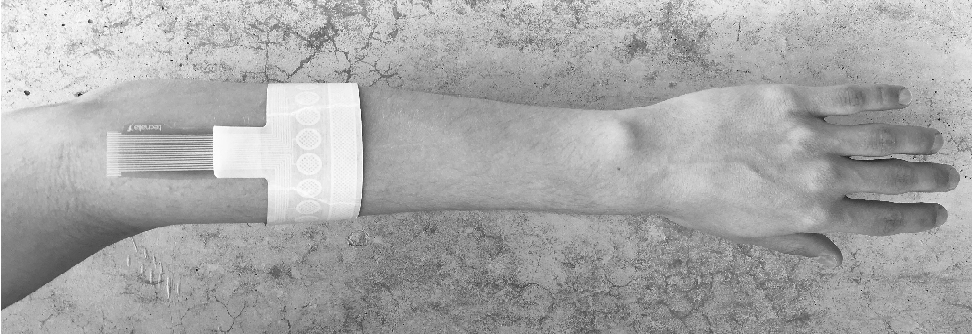
\includegraphics[width=0.85\textwidth]{figures/elec_place}  
	\caption{Illustration of the placement of the electrode array.}
	\label{fig:meth:elec_place} 
\end{figure}

In order to provide meaningful sensory feedback to the subject, a range of distinguishable sensory thresholds had to be determined for the subject. As presented in \secref{sec:vp} the virtual prosthesis had a range of one to four states. Hence, four thresholds based on amplitude values were determined to accommodate four levels of feedback in the amplitude scheme. Furthermore, since the sensory sensitivity varies across different locations of the circumference of the arm, the sensory thresholds had to be determined for each individual pad in the electrode armband. Sensory thresholds were found by slowly increasing the amplitude while fixating the pulse width and frequency at 500 $\mu s $ and 50 Hz, respectively. \\
In the first round, the lowest threshold was determined, which from now on will be referred to as the perception threshold. For each pad, the amplitude was set to start at 0 $\mu A $ and then increase in steps of 100 $\mu A $ per second. The subject was instructed in reporting when electrical stimulation could be sensed and that the subject was sure the activated pad was the origin of the perceived stimulation. The pad was deactivated and reactivated once more with the reported sensory threshold amplitude for a second verification. This process was carried out for each pad starting from pad 1 to 16. Subsequently, the subject was presented with the determined amplitudes in each pad, such that the sensation in the current pad was compared to the neighboring pad. This was carried out such that the determined amplitudes could be readjusted to achieve more homogeneous sensations across all pads.  \\
In the second round, the fourth level thresholds, referred to as tolerance threshold, were determined using the same procedure as in round one. The tolerance threshold was defined at highest amplitude the subject felt pleasant. The starting amplitude was in this round, however, the perception threshold. The amplitude was set to increase in steps of 200 $\mu A $ per second. The amplitude was increased until the subject reported that the threshold was reached, the stimulation was causing functional muscle activation or a maximum of 10000 $\mu A $ was reached. Again the intensities were readjusted to achieve homogeneous sensations. Throughout the process of determining the sensory thresholds, the subject was placed facing away from the computer screen to avoid bias from seeing the used amplitude values.  \\ 
Using the determined perception and tolerance thresholds, the second and third level thresholds were calculated for the $i^{th}$ pad as the following:

\begin{equation}
2~lvl(i) = perception(i) + (\frac{1}{3} \cdot (tolerance(i) - perception(i)))
\end{equation}

\begin{equation}
3~lvl(i) = tolerance(i) - (\frac{1}{3} \cdot (tolerance(i) - perception(i)))
\end{equation}


       